\section {Sincronização via \textit{Ethernet} com a \textit{BeagleBone Black}}

\subsection {Introdução}

A sincronização dos diversos componentes presentes no sistema de controle de um
acelerador de partículas é um fator fundamental para seu bom funcionamento. Os
sistemas que necessitam de sincronismo, como as fontes de corrente para os imãs,
controladores de feixe e de injeção, devem exercer as suas
respectivas funções em momentos especificados por pulsos de sincronismo, que
podem ser enviados, por exemplo, por geradores de sinais espalhados pela
infraestrutura local. A precisão com que estes equipamentos recebem tais pulsos
depende de diversas variáveis, como o tipo de canal de comunicação
utilizado no envio do pulso e a interface de entrada de dados que eles possuem.
A precisão pode ser obtida através da medição do \textit{jitter}, ou
desvio-padrão, do \textit{delay} calculado entre o envio do pulso e a sua
recepção no equipamento.
O \textit{Sirius}, por exemplo, possui especificações para diversos sistemas de
sincronismo, que variam de acordo com a necessidade de precisão dos equipamentos
e das funções desempenhadas por eles. Para casos mais graves, como o da bomba de
elétrons do acelerador linear (\textit{LINAC}), os \textit{jitters} não podem
ultrapassar os \textit{50ps} e soluções especiais devem ser exploradas, como a
implementação de uma rede \textit{WhiteRabbit}, que está sendo
desenvolvida e estudada por outros laboratórios no mundo todo.

\vspace{12pt}

Um sistema de sincronismo para as fontes de corrente já
foi implementado pelo grupo de controle, utilizando as unidades
\textit{Programmable Realtime Unit}, ou simplesmente \textit{PRU}, presentes na
\textit{BeagleBone}. Tais unidades apresentam \textit{clock} de 200MHz,
núcleos de memória própria e compartilhada, e módulos dedicados, como o
\textit{Enhanced GPIO}, que favorecem a implementação de aplicações
\textit{realtime}, em que a precisão é uma necessidade importante. Soluções
implementadas para a \textit{PRU} não estão sujeitas a fatores que degradam a
precisão como o compartilhamento de \textit{CPU} com outros
processos e preeempção. Aplicações que rodam sobre \textit{Linux} embarcado e
que, portanto, compartilham recursos com outros processos, apresentam,
geralmente, desempenho inferior. O sistema desenvolvido anteriormente pelo grupo
utiliza a \textit{PRU} para a recepção do sinal de sincronismo e ativa, posteriormente, seus nós
escravos, conforme figura \ref{fig:pru_sincronismo} abaixo. Esse sistema obteve
um \textit{jitter} da ordem de 15ns, representando, assim, um valor próximo do
ótimo, uma vez que os ciclos de processamento de cada um dos componentes estão
próximos de 5ns.

\begin{figure}[h]

\centering
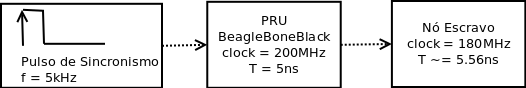
\includegraphics[scale=0.65]{image/pru_bbb_sincronismo}
\caption {Esquema de sincronismo realizado pelo grupo de controle.}
\label{fig:pru_sincronismo}
\end{figure}

\vspace{12pt}

Nesta seção, será apresentada a alternativa descrita na figura
\ref{fig:pru_sincronismo_ethernet}, que utiliza o protocolo \textit{Ethernet} e
equipamentos padrões na implementação deste tipo de rede, como
\textit{switches}, para o envio dos \textit{triggers} de sincronismo, e a sua
respectiva \textit{performance}. Duas implementações deste modelo serão
discutidas: uma em que tanto \textit{BB1} quanto \textit{BB2} executam
programas no \textit{kernel space}, chamados de \textit{kernel modules}, e a
outra, em que ambas utilizam seus módulos PRUs.

\vspace{12pt}

\begin{figure}[h]

\centering
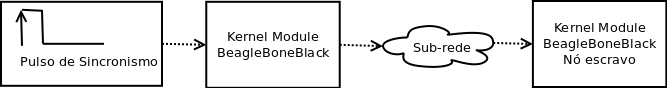
\includegraphics[scale=0.65]{image/pru_bbb_sincronismo_ethernet}
\caption {Sistema de sincronismo proposto.}
\label{fig:pru_sincronismo_ethernet}
\end{figure}

\subsection {Implementação de \textit{Kernel Modules}}

Esta subseção é dedicada à primeira implementação do sistema de sincronismo
proposto.

\subsubsection{\textit{Loadable Kernel Modules}}

% A principal diferença entre os dois sistemas apresentados na subseção anterior é
% que, no segundo, não utilizamos a unidade \textit{PRU} da \textit{BeagleBone
% Black}. 
Nesta seção, propomos desenvolver módulos do
\textit{kernel} do \textit{Linux}, chamados de \textit{Loadable Kernel Modules} (\textit{LKM}).
Tais módulos são mecanismos que permitem a adição ou remoção de código do \textit{Linux kernel}
em tempo de execução e, por esta razão, são ideais para a implementação de
\textit{device drivers} \cite{derek}, cujo propósito principal é realizar a
comunicação com o \textit{hardware} disponível.  

\vspace{12pt}

Sendo essencialmente parte do \textit{kernel}, os \textit{LKMs} são executados
no \textit{kernel space} e, por isso, possuem endereços de memória e
\textit{APIs} próprios, que são, por sua vez, separados daqueles
disponíveis no \textit{user space}. Este último representa o \textit{space} em
que, na maioria das vezes, escrevemos e executamos as aplicações em C. A figura
\ref{fig:derek_kernel_user} resume as interações entre os dois espaços: o
\textit{user space} comunica-se com \textit{kernel space} através de
\textit{system calls}, que, por sua vez, acessa o \textit{hardware} através de
\textit{drivers} específicos. O \textit{kernel space} possibilita o tratamento
de interrupções, que serão utilizadas neste exemplo, ao contrário do
\textit{user space}.

\begin{figure}[h]

\centering
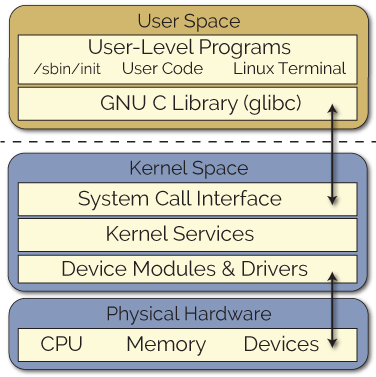
\includegraphics[scale=0.45]{image/userspace-kernelspace}
\caption {Comunicação entre \textit{kernel} e \textit{user spaces}. Extraída de
\cite{derek}.}
\label{fig:derek_kernel_user}
\end{figure}

\subsubsection{Descrição das características do projeto}

Neste projeto, utilizou-se duas \textit{BeagleBones Black}, denominadas
\textit{BB1} e \textit{BB2}, conforme figura \ref{fig:pru_sincronismo_ethernet}.
De maneira geral, foram desenvolvidas duas aplicações, uma para a \textit{BB1},
cujas funções são receber o \textit{trigger} de sincronismo e preparar o pacote
\textit{UDP} para envio, e a outra, para a \textit{BB2}, responsável pela
recepção do respectivo pacote e tratamento.
A aplicação que recebe o \textit{trigger} mantém um contador interno e o
transmite em intervalos definidos de tempo, para que o nó escravo possa também
manter um contador de mesmo tipo. Dessa forma, o nó escravo pode determinar se
um pacote foi perdido durante a transmissão e corrigir seu contador.

\vspace{12pt}

Em termos de programação, as aplicações apresentam as seguintes características:

\begin{itemize} \renewcommand\labelitemi{--}
  \item \textit{Kernel Module} em \textit{BB1}: um \textit{timer} gera
  interrupções a cada 1ms. Na rotina de tratamento desta interrupção, um
  registro contendo os dados a serem enviados via \textit{Ethernet} é
  adicionado em um \textit{buffer} circular. Uma outra \textit{thread}
  é responsável por retirar estes elementos do \textit{buffer}, prepapar os
  pacotes \textit{UDP} e enviá-los.

  \item \textit{Kernel Module} em \textit{BB2}: uma \textit{thread} é
  instanciada e espera pacotes \textit{UDP}. Quando recebe, atualiza seu
  contador e seus pinos de saída.
\end{itemize}

Por questões de simplicidade, o módulo \textit{PWM} da placa que envia os
pacotes \textit{UDP} (\textit{BB1}) será utilizado como gerador dos
\textit{triggers} de sincronismo. 

% \subsubsection {Configuração do \textit{PWM} com o \textit{Device Tree
% Overlays}}
% 
% Os mecanismos de \textit{Cape Manager} e \textit{Device Tree Overlays} permitem
% a modificação do sistema, como, por exemplo, configuração da função dos pinos,
% ativação e carregamento de módulos em tempo de execução a partir de programas
% sendo executados no \textit{user space}.
% 
% \vspace{12pt}
% 
% 
% Sendo assim, a fim de modificarmos o pino \texttt{P9\_22} (\textit{header P9},
% pino 22) para que atue como uma saída do módulo \textit{PWM}, é necessário
% escrevermos um arquivo de extensão \texttt{.dts} (\textit{device tree source}),
% contendo as especificações que desejamos adotar. Um arquivo deste tipo é
% disponível em \url{http://tinyurl.com/ntkl2w7} e contem todas as possíveis
% configurações de todos os pinos da \textit{BeagleBone Black}. Como vamos
% utilizar somente as linhas referentes ao \texttt{P9\_22}, podemos copiá-las para
% um arquivo separado e adotá-lo em seguida. Após obtermos tal arquivo, é
% necessário compilá-lo a partir do comando \texttt{dtc} e incluir o resultado no
% diretório \texttt{/lib/firmware/}.
% 
% \vspace{12pt}
% 
% Para carregar o \textit{overlay}, configuramos duas variáveis de ambiente:
% 
% \begin{lstlisting}[keywordstyle=\ttfamily, style=nonumbers]
% $ export SLOTS=/sys/devices/bone_capemgr.9/slots
% $ export PINS=/sys/kernel/debug/pinctrl/44e10800.pinmux/pins
% \end{lstlisting}
% 
% \vspace{12pt}
% 
% Executamos, então, os comandos abaixo, em que \texttt{pwm\_P9\_22} referencia o
% arquivo gerado após compilação. \texttt{duty\_ns} e \texttt{period\_ns}
% são utilizados, respectivamente, para configurar o intervalo de tempo em que a
% onda permanecerá em nível lógico alto e o seu período total. Para as próximas
% seções, vamos adotá-los como, respectivamente, 2\textit{ms} e 70\textit{ms}. Um
% \textit{script bash}, que pode ser encontrado no repositório do grupo, foi
% escrito e automatiza o processo abaixo.
% 
% \begin{lstlisting}[keywordstyle=\ttfamily, style=nonumbers]
% $ echo pwm_P9_22 > $SLOTS
% $ echo pwm > /sys/devices/ocp.3/P9_22_pinmux.12/state
% $ cd /sys/class/pwm/
% $ echo 0 > export 
% $ cd pwm0/
% $ echo 2000000 > duty_ns
% $ echo 70000000 > period_ns
% \end{lstlisting}

\subsubsection{Implementação do \textit{Kernel Module} de \texttt{BB1}}
\label{sec:bb1}

O \textit{module} desenvolvido para a placa \texttt{BB1} instancia duas
\textit{threads}: uma para inicialização dos componentes e a outra para
processamento e envio de pacotes \textit{UDP}. No \textit{kernel space}, cada
\textit{thread} é definida por uma estrutura do tipo \texttt{struct
task\_struct}, especificada na biblioteca \texttt{linux/kthread.h}, que provê também as funções
\texttt{kthread\_create} e \texttt{wake\_up\_process}. A primeira é reponsável
por alocar os recursos necessários à execução de uma \textit{thread} e a
segunda, por permitir a sua execução. É possível alterar a prioridade e a
\textit{policy} de uma \textit{thread} através da função
\texttt{sched\_setscheduler}, disponível em \texttt{linux/sched.h}. Esses dois
parâmetros são usados pelo \textit{Linux scheduler} para decidir qual dos
processos interrompidos deterá o processador após a interrupção ou bloqueio do
processo em curso de execução. O \textit{Linux} fornece duas políticas de
\textit{real-time}, \texttt{SCHED\_FIFO} e \texttt{SCHED\_RR}, que possuem
prioridade superior à politíca comum, \texttt{SCHED\_NORMAL}. Processos cujas
\textit{scheduler classes} são do tipo \textit{real-time} sempre são escolhidos
antes daqueles de política comum. É necessário observar que,  no \textit{kernel}
padrão do \textit{Linux},  estas classes não são capazes de garantir um
comportamento dito \textit{hard real-time} \cite{linuxlove}, isto é, que
asseguram o cumprimento de qualquer requisito dentro de um certo limite. As
\textit{real-time scheduling policies} fornecem, portanto, um comportamento de
\textit{soft real-time}, ou seja, o \textit{kernel} faz o máximo possível para
atender às requisições, mas não pode prometer sempre cumpri-las. Dada tal
limitação, um \textit{patch}, chamado \path{RT_PREEMPT} e disponível em
\cite{rt}, foi desenvolvido para garantir características de \textit{hard real-time}. Quando
uma tarefa do tipo \texttt{SCHED\_FIFO} assume a \textit{CPU}, ela continua a
ser executada até que ela seja bloqueada ou que ela conceda explicitamente o
processador a outro processo, podendo rodar indefinidamente caso nenhuma dessas
condições seja atendida. Somente uma tarefa \texttt{SCHED\_FIFO} ou
\texttt{SCHED\_RR} de maior prioridade pode interromper sua execução. Para as
tarefas do tipo \texttt{SCHED\_RR}, o princípio é o mesmo, porém elas são
submetidas a um intervalo de execução, sendo que, ao fim deste intervalo, tais
tarefas perdem os recursos de processamento e entram na fila circular de espera.
Em outras palavras, a política \texttt{SCHED\_RR} é semelhante à
\texttt{SCHED\_FIFO}, exceto no tempo que é permitido ao uso de \textit{CPU}. No
nosso caso, ambas as \textit{threads} terão políticas de \texttt{SCHED\_FIFO},
mas aquela que é interrompida pelo \textit{timer} e
\textit{GPIOs} possuirá maior prioridade. Em adição, a segunda \textit{thread}
(aquela responsável pelo envio de pacotes) desiste da \textit{CPU} quando o
\textit{buffer} circular está vazio e só é \textit{acordada} quando uma
interrupção de tempo ocorrer (o \textit{buffer} volta a ser preenchido na função de
tratamento desta interrupção). Os fluxogramas da figura \ref{fig:threads_bb1}
resumem o funcionamento destas \textit{threads}.

\vspace{12pt}

A figura \ref{fig:thread_int} especifica o fluxograma da \textit{thread\_int}
que preenche o \textit{buffer} circular a cada interrupção do relógio e sinaliza
para a \textit{thread\_proc} que ele não está mais vazio. A figura
\ref{fig:thread_proc} evidencia que um pacote é enviado somente o
\textit{buffer} não estiver vazio. Caso contrário, a \textit{thread\_proc}
se bloqueia esperando uma interrupção do relógio. As funções \texttt{wake\_up} e
\texttt{wait\_event} estão disponíveis na biblioteca \texttt{linux/wait.h}. A
segunda deve receber como parâmetro uma fila, que representa a estrutura de
dados onde serão colocados os processos que esperam pelo evento. Essa fila é do
tipo \texttt{wake\_queue\_head\_t} e pode ser criada estaticamente, via
a \textit{macro} \texttt{DECLARE\_WAITQUEUE()}, ou dinamicamente, via a função
\texttt{init\_waitqueue\_head()}.

	\begin{figure}[h!]
	
	\centering
	
		\begin{subfigure}{.33\textwidth}
		  \centering
		  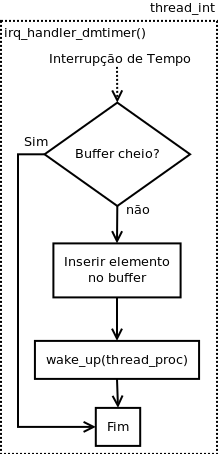
\includegraphics[scale=0.55]{image/thread_int}
		  \caption{\centering Fluxograma da \textit{thread} que é interrompida pelo
		  \textit{timer} de \texttt{BB1}.}
		  \label{fig:thread_int}
		  
		\end{subfigure}%
		\begin{subfigure}{.33\textwidth}
		  \centering
		  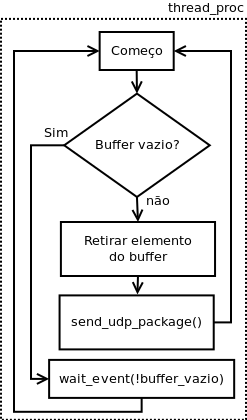
\includegraphics[scale=0.55]{image/thread_proc}
		  \caption{\centering Fluxograma da \textit{thread} que envia pacotes à
		  rede de \texttt{BB1}.}
		  \label{fig:thread_proc} 
		\end{subfigure}%
		\begin{subfigure}{.33\textwidth}
			\centering
			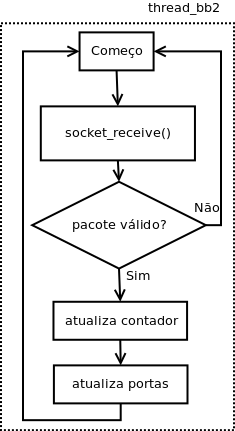
\includegraphics[scale=0.55]{image/thread_bb2}
			\caption {\centering Fluxograma da \textit{thread} do \textit{kernel module}
			em
			\texttt{BB2}.}
			\label{fig:thread_bb2}
		\end{subfigure}%
		\caption{Fluxogramas das \textit{threads} que compõem \texttt{BB1}
		e \texttt{BB2}.}
		\label{fig:threads_bb1}
		\end{figure} 

\vspace{12pt}

Os processadores da família \textit{Sitara AM335x} da \textit{Texas Instruments}
possuem um módulo, chamado de \textit{DMTimer}, composto por 7 \textit{timers}
configuráveis. Cada um dos \textit{timers} contém um contador de 32
\textit{bits} crescente com capacidade de \textit{auto reload} e geração de
interrupção ao atingir seu valor máximo (\texttt{0xFFFFFFFF}), isto é, em caso
de \textit{overflow}. Além disso, é possível configurar um divisor de frêquencia
(\textit{prescaler}) e escolher o sinal de \textit{clock} que será usado pelo
componente. No \textit{kernel space}, a biblioteca \texttt{plat/dmtimer.h}
fornece as principais operações para configuração do módulo. 

\vspace{12pt}

A função \texttt{omap\_dm\_timer\_request()} retorna uma estrutura do tipo
\texttt{struct omap\_dm\_timer} que representa um dos \textit{timers}
disponíveis no módulo. Há mais algumas variantes desta chamada, porém a
principal é a \texttt{omap\_dm\_timer\_request\_specific(int timer\_id)}, que
recebe como parâmetro o \textit{id} do \textit{dmtimer} desejado. É necessário
notar, porém, que talvez seja necessário a configuração de um \textit{overlay}
para a configuração dos pinos utilizados pelo respectivo \textit{timer}. Em
seguida, executamos a chamada \path{omap_dm_timer_set_source}, que
configura o sinal de \textit{clock} de entrada. Utilizamos o \textit{clock} de
32kHz, portanto passamos a constante \texttt{OMAP\_TIMER\_SRC\_32\_KHZ} como
parâmetro à função. \texttt{omap\_dm\_timer\_set\_prescaler} permite definir o
valor do divisor de frequência e \path{omap_dm_timer_set_load_start}, o
valor que será carregado no contador quando um \textit{overflow} ocorrer. Tais
definições dependem do intervalo desejado entre interrupções e são dadas pela
equação \ref{eq:timer}, em que \textit{TDLR} é o valor a ser carregado no
contador, \textit{PTV}, o \textit{prescaler} e \(f_{clock}=32kHz\).

\begin{equation} 
t = (\text{0xFFFFFFFF} - TDLR + 1)*\frac{1}{f_{clock}}*2^{PTV+1}
\label{eq:timer}
\end{equation}

No nosso caso, desejamos interrupções a cada \(t=1ms\) com \(PTV=1\). A
aplicação direta da equação \ref{eq:timer} resulta em \textit{TDLR} =
0xFFFFFFF7.

\vspace{12pt}

O último passo é ativar a interrupção em caso de \textit{overflow} e associar a
ela uma função de tratamento. Para configurá-la, utilizamos três funções:

\begin{itemize} \renewcommand\labelitemi{--}
  \item \texttt{omap\_dm\_timer\_get\_irq()}: retorna o \textit{id} da
  interrupção associada ao \textit{timer} passado como parâmetro;

  \item \texttt{omap\_dm\_timer\_set\_int\_enable()}: habilita interrupção no
  módulo. Recebe como parâmetro uma constante que define o evento que deve ser
  associado à interrupção. No nosso caso, como queremos que uma interrupção seja
  lançada após \textit{overflow} do contador, passamos o valor
  \path{OMAP_TIMER_INT_OVERFLOW};

  \item \texttt{request\_irq()}, da biblioteca \texttt{linux/interrupt.h}:
  recebe como parâmetro o \textit{id} da interrupção, a sua função tratadora e
  o tipo de função. Este último é uma constante definida na biblioteca e vale
  \path{IRQF_TIMER}. No nosso caso, criamos uma função chamada
  \path{dmtimer_irq_handler()} que retorna uma estrutura do tipo \texttt{irqreturn\_t}. Para comunicar ao sistema
  operacional que a interrupção foi corretamente tratada, tal função deve
  retornar \texttt{IRQ\_HANDLED}. Além desta constante, a função deve atualizar
  o registrador de \textit{status} do módulo realizando uma escrita. Isso é
  feito através da função \texttt{omap\_dm\_timer\_write\_status()}, com o
  parâmetro \path{OMAP_TIMER_INT_OVERFLOW}.
\end{itemize}
 
Enfim, iniciamos o \textit{timer} com a chamada de \path{omap_dm_timer_start()}.

\vspace{12pt}

A próxima etapa é a configuração dos pinos de entra e saída. A biblioteca
\texttt{linux/gpio.h} fornece as funções necessárias para definirmos a direção
(entrada ou saída) e o nível lógico a ser atribuído a um respectivo pino.
Utilizamos dois pinos de entrada e saída nesta aplicação:

\begin{itemize} \renewcommand\labelitemi{--}
  \item \texttt{GPIO\_48} (\texttt{P9\_15}): pino de entrada que recebe o
  \textit{trigger} de sincronismo. A cada borda de subida detectada, uma
  interrupção é lançada e algumas \textit{flags} responsáveis por armazenar a
  ocorrência do evento são atualizadas. Quando a \textit{thread\_proc} prepara o
  próximo pacote, ela consulta essas \textit{flags} e, caso estejam
  \textit{setadas}, adiciona ao respectivo pacote o \textit{trigger} recebido;

  \item \texttt{GPIO\_68} (\texttt{P8\_15}): pino de saída que tem seu valor
  alterado quando um \textit{trigger} de sincronismo foi detectado. Utilizado
  para testes da aplicação.
\end{itemize}

Para verificar se um pino pode ser utilizado, chamamos a função
\path{gpio_is_valid}, cujo parâmetro é o \textit{id} do respectivo pino. Se o
retorno for diferente de 0, o \textit{id} é valido e podemos continuar a
configurá-lo. Em seguida, executamos, em sequência,
\path{gpio_request()}, \path{ gpio_direction_output()} - para saída - ou
\path{gpio_direction_input()} - para entrada - e \path{gpio_export()}. Tais
funções são responsáveis por, respectivamente, reservar o pino, configurar sua
direção e exportá-lo, permitindo ou não que outras aplicações o utilizem. O pino
de entrada requer adicionalmente que uma interrupção seja relacionada a ele.
Para tal, repetimos o procedimento realizado para o \textit{timer}, isto é,
obtemos o \textit{id} da interrupção através de \path{gpio_to_irq()} e associamos
uma função tratadora com \path{request_irq()}. Entretanto, ao invés de enviarmos
o parâmetro \path{IRQF_TIMER} para esta última, passamos
\path{IRQF_TRIGGER_RISING}, que lançará as interrupções quando bordas de subida
forem detectadas. Em relação aos pinos de saída, utiliza-se 
\path{gpio_set_value()} para modificar o valor de tensão imposta na respectiva
saída, cujo \textit{id} é passado como parâmetro à função. Os recursos
utilizados por um pino de entrada ou saída são liberados a partir das chamadas
\path{gpio_unexport()} e \path{gpio_free()}.

\vspace{12pt}

Enfim, o último aspecto a ser discutido neste módulo é a implementação do envio
de pacotes \textit{UDP}. Três bibliotecas devem ser importadas a fim de realizar
essa comunicação: \path{linux/netdevice.h}, \path{linux/ip.h} e
\path{linux/in.h}. O primeiro passo é a criação do \textit{socket} de
comunicações, que é realizado pela chamada à função \path{sock_create()},
passando como parâmetros algumas constantes e a estrutura \texttt{struct socket}
que representa um \textit{socket} no \textit{kernel space}. As constantes
especificam o tipo do respectivo \textit{socket}, sendo que, para aplicações
\textit{UDP}, utilizamos \path{AF_INET}, \path{SOCK_DGRAM} e \path{IPPROTO_UDP},
que especificam, respectivamente, o formato dos endereços (endereços
\textit{Internet Protocol v4}), as camadas de transporte e rede dos pacotes a
serem enviados. Em seguida, definimos seu endereço e a porta a partir da função
\path{connect()}, que pode ser acessada através do atributo \path{ops} de
\texttt{struct socket}. Além do \textit{socket} criado, ela recebe como
parâmetro um ponteiro para uma variável do tipo \texttt{struct sockaddr}, que,
por sua vez, possui três atributos importantes: \path{sin_family},
\path{sin_addr.s_addr} e \path{sin_port}. Recebem, respectivamente,
\path{AF_INET}, \path{htonl(INADDR_SEND)} e \path{htons(CONNECT_PORT)}, em que
\path{htonl()} e \path{htons()} são funções pré-definidas que convertem valores
de \textit{host order} para \textit{network byte order} (\path{0xc0a80216} para
\path{192.168.2.22}, por exemplo), \path{INADDR_SEND} é o endereço para o qual
deseja-se enviar datagramas e \path{CONNECT_PORT} é a porta.
\path{connect()}, além de definir tais características, também ativa a conexão
no \textit{socket}. O envio de pacotes é realizado por \path{sock_sendmsg()},
que recebe dois parâmetros: as estruturas \texttt{struct socket} e
\texttt{struct msghdr}, que contém o conteúdo da mensagem. Enfim, para desalocar
o \textit{socket}, chama-se a funçao \path{sock_release()}.

% \vspace{12pt}
% 
% Por fim, a compilação do arquivo \path{.c} é realizada por meio de um
% \textit{Makefile}, cujo conteúdo é semelhante ao código abaixo, em que
% \path{timer_kernel_module} é o nome do arquivo do módulo e \texttt{\$(shell
% uname -r)} retorna a versão dos \textit{linux headers} instalados na
% \textit{Beagle}.
% 
% \begin{lstlisting}[keywordstyle=\ttfamily, style=nonumbers]
% obj-m+=timer_kernel_module.o 
%  
% all:
% 	make -C /lib/modules/$(shell uname -r)/build/ M=$(PWD) modules 
% clean:
% 	make -C /lib/modules/$(shell uname -r)/build/ M=$(PWD) clean
% \end{lstlisting}

% \vspace{12pt}
% 
% A adição do módulo compilado (arquivo \path{.ko}) é realizado através do comando
% \path{insmod} e a sua remoção, a partir de \path{rmmod}. O arquivo
% de \textit{log} pode ser utilizado para eventual \textit{debug}, sendo acessado
% a partir de \path{/var/log/kern.log}.

\subsubsection{Implementação do \textit{Kernel Module} de \texttt{BB2}}

Uma só \textit{thread} é instanciada no \textit{kernel module} de \texttt{BB2}.
Ela aguarda a recepção de pacotes \textit{UDP} e os processa. Ela é criada da
mesma forma descrita na subseção anterior e tem sua \textit{policy} modificada
para \path{SCHED_FIFO}, a fim de obter tratamento de \textit{real-time}. O
fluxograma da figura \ref{fig:thread_bb2} destaca a execução do módulo. Quando
um pacote é recebido, há uma verificação de sua integridade e, caso seja válido,
o contador e as portas de \textit{gpio} são atualizadas conforme conteúdo.
Observa-se que o processo de inicialização de tais portas segue o mesmo
princípio que o descrito em \textbf{Implementação do \textit{Kernel Module} de
\texttt{BB1}}. A criação do \textit{socket}, no entanto, é ligeiramente
diferente: ao invés da função \path{connect()}, utiliza-se \path{bind()}, que
atribui um endereço e porta ao respectivo \textit{socket}, passado como
parâmetro através de uma estrutura do tipo \texttt{struct sockaddr}, que é
inicializada com as funções \texttt{htonl} e \texttt{htons}, destacadas
anteriormente. A recepção dos pacotes é feita via \path{sock_recvmsg()}, que
bloqueia a \textit{thread} até que um datagrama seja detectado.
% 
% \vspace{12pt}
% 
% A compilação pode ser feito através de um \textit{Makefile} e a adição e remoção
% do módulo, via os comandos \path{insmod} e \path{rmmod}.


\subsection{Utilizando o módulo PRU}

Implementações alternativas para os \textit{kernel modules} de \textit{BB1} e
\textit{BB2} foram propostas usando o módulo PRU da \textit{BeagleBone Black}.
Para \textit{BB1}, a configuração do \textit{timer} e a verificação das
interrupções geradas por ele e pelo pulso de sincronismo são feitas pela PRU.
Quando um \textit{trigger} é recebido, um sinal é enviado para um programa
rodando no \textit{user space} da \textit{Beagle}, cujo propósito é, de fato,
enviar pacotes \textit{UDP} para \textit{BB2}. É importante observar que a
comunicação entre o processador e o módulo PRU é garantida via \textit{hardware}
e que uma API contendo funções de comunicação com a PRU também é fornecida pela
comunidade.

\vspace{12pt}

Um processo semelhante foi realizado para \textit{BB2}, isto é, substituiu-se o
\textit{kernel module} por um programa rodando na unidade de tempo real. Tal
programa verifica, através de \textit{polling} nos registradores do controlador
de rede, se um novo pacote foi recebido. Se isto ocorreu, então um sinal é
enviado a um outro programa no \textit{user space}, responsável por tratar tal
pacote. O tratamento de tal pacote não é realizado diretamente na PRU, visto que
seria necessária a implementação de toda a pilha \textit{UDP/IP}.

\subsection {Resultados}

Para avaliar os resultados, conectamos o \textit{PWM} ao canal 3 do osciloscópio
e configuramos o \textit{trigger} para detectar subidas de borda deste canal. O
módulo de \texttt{BB2} foi configurado para modificar o estado de um pino de
saída, ao qual conectamos ao canal 2, a fim de gerar um simples pulso quando um
pacote contendo um \textit{trigger} de sincronismo for recebido. Dessa forma,
podemos avaliar o \textit{delay} entre a criação do evento inicial e de sua
recepção no nó escravo, assim como o \textit{jitter} associado. Para tal,
utilizamos a ferramenta \textit{Histograma} disponibilizada no equipamento e a
configuramos para adquirir medidas relacionadas ao canal 2, isto é, pulsos
gerados pela \textit{Beagle} \texttt{BB2}. Modificamos a opção \textit{Tempo de
Persistência} do \textit{Display Forma de onda} para infinito, de forma a
garantir que a tela do osciloscópio mantenha os pulsos gerados em instantes
anteriores. Enfim, habilitamos o funcionamento do osciloscópio, obtendo o
resultado presente na figura \ref{fig:osciloscopio_thread} para a implementação
contendo os \textit{kernel modules} e na \ref{fig:pru_osciloscopio_thread} para
a implementação utilizando a PRU. Os desvios padrões, ou \textit{jitters},
obtidos são, respectivamente, 5.7\textit{ms} e 985.1\(\mu s\), muito distantes
daquele adquirido pelo sistema construído pelo grupo de controle, no qual
utilizou-se somente a \textit{PRU} e obteve-se um valor próximo de
15\textit{ns}. Tal diferença é explicada, basicamente, por dois fatores: o canal
utilizado para envio da mensagem e o componente de processamento da
\textit{Beagle}. Nas nossas aplicações, utilizamos um \textit{switch HP V1810G},
que apresenta um comportamento \textit{não determinístico}, isto é, não é
possível prever com certitude o tempo necessário para que um pacote seja
entregue a um determinado \textit{host}. O segundo aspecto a ser considerado é
que aplicações rodando na \textit{PRU} não dividem recursos com outros
processos, ao contrário de aplicações que rodam em \textit{embedded linux}. Na
seção \ref{sec:bb1}, comentamos que, apesar do \textit{Linux} fornecer políticas
de preempção \textit{real-time}, o comportamento chamado de \textit{hard
real-time} não poderia ser alcançado pelo \textit{kernel}. Em oposição, as
unidades \textit{PRUs} da \textit{Beagle} foram desenvolvidas para este
propósito.

\begin{figure}[h]

\centering
	\begin{subfigure}[t]{0.5\textwidth}
		\centering
		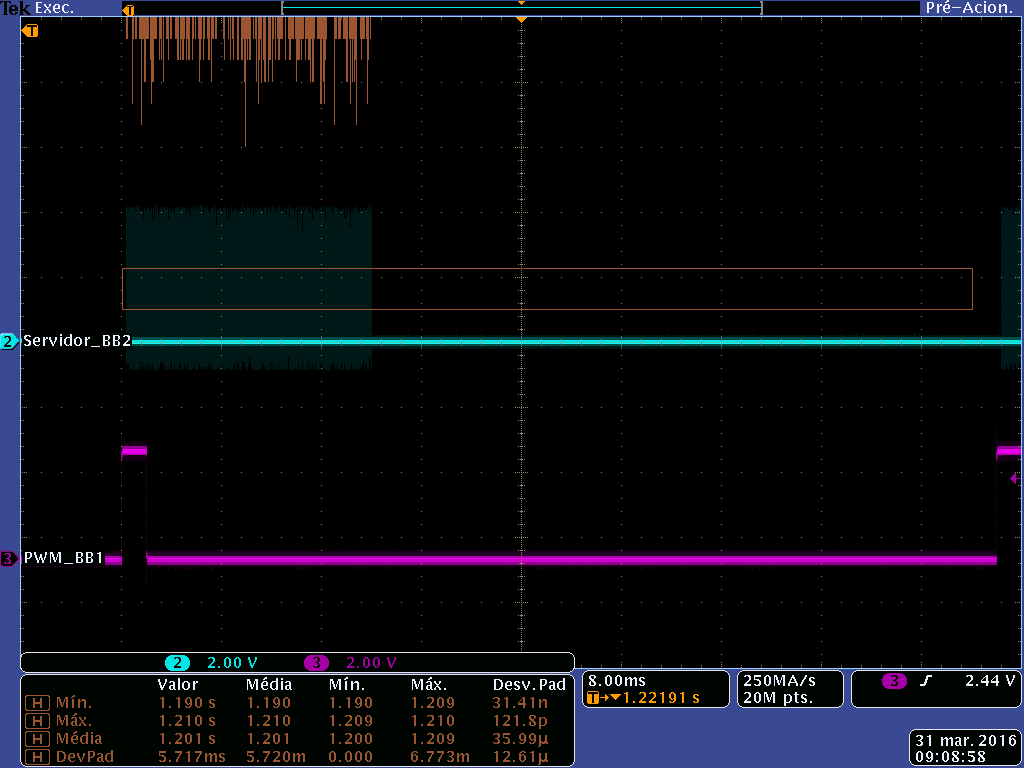
\includegraphics[width=0.95\textwidth]{image/tek_com_threads}
		\caption {\centering Captura de tela do osciloscópio para a implementação com
		\textit{kernel modules}.}
		\label{fig:osciloscopio_thread}
	\end{subfigure}%
	\begin{subfigure}[t]{0.5\textwidth}
		\centering
		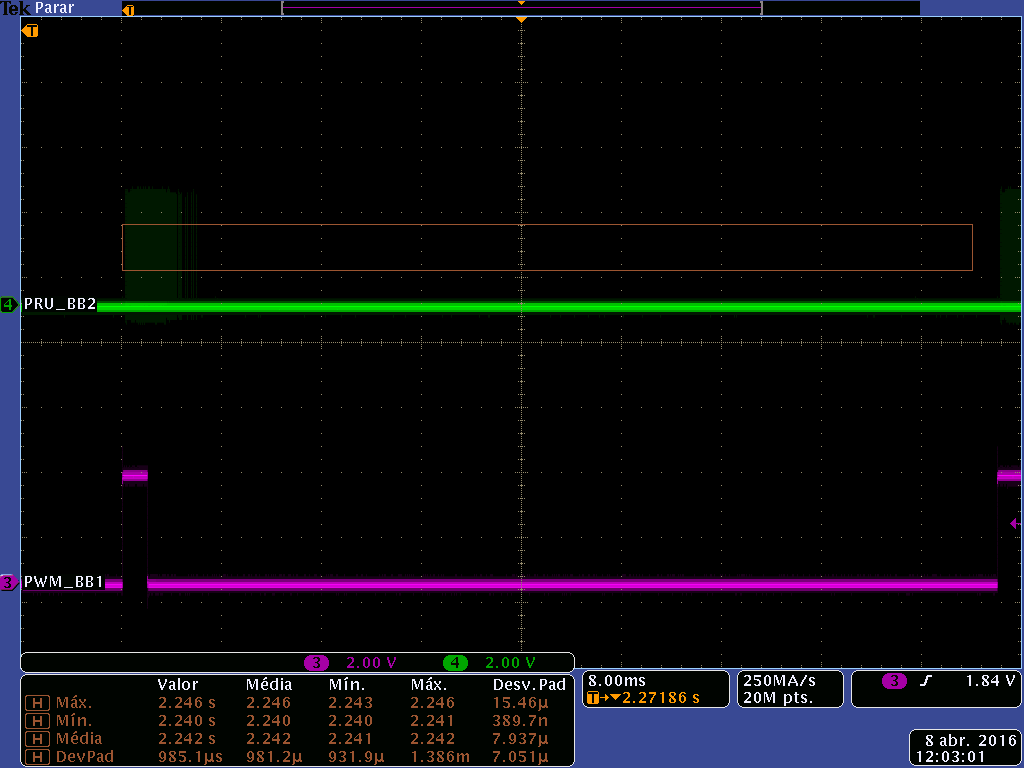
\includegraphics[width=0.95\textwidth]{image/tek_pru}
		\caption {\centering Captura de tela do osciloscópio para implementação com
		PRU.}
		\label{fig:pru_osciloscopio_thread}
	\end{subfigure}%
	
	\caption {Resultados encontrados para as duas implementações.}
\end{figure}

\subsection{Alternativa de solução: \textit{Industrial Ethernet}}

Alguns protocolos foram desenvolvidos a fim de alcançar exigências de
\textit{hard real-time} sobre redes \textit{Ethernet}. Um deles é o
\textit{EtherCAT} (\textit{Ethernet for Control Automation Technology}),
desenvolvido pela empresa alemã \textit{Beckhoff}, que utiliza as unidades de
processamento \textit{real-time} (\textit{PRUs}). Um dos incovenientes desta
aplicação em relação à \textit{BeagleBone Black} é que o seu processador,
\textit{Sitara AM3358}, não suporta este protocolo, sendo que os únicos da mesma
família que o suportam são \textit{AM3357} e \textit{AM3359}. A \textit{Texas
Instruments} fornece um \textit{kit} de desenvolvimento com o último, chamado de
\textit{AM3359 Industrial Communications Engine}, e uma biblioteca desenvolvida
para o uso deste protocolo, \textit{SYS/BIOS Industrial Software Development Kit
(SDK)}. Além do \textit{EtherCAT}, outras alternativas para comunicação
\textit{real-time} sobre \textit{Ethernet} e que são suportadas pelo processador
AM3358 são \textit{Ethernet/IP}, \textit{PROFINET RT/IRT} e \textit{PROFIBUS}.
